\documentclass[a4paper]{article}

\usepackage[english]{babel}
\usepackage[utf8]{inputenc}
\usepackage{amsmath}
\usepackage{graphicx}
\usepackage[colorinlistoftodos]{todonotes}
\usepackage{algorithmicx}
\usepackage[ruled,vlined]{algorithm2e}
\title{Data Mining project report}

\author{Lorenzo Paciotti}

\date{\today}

\begin{document}
\maketitle

\begin{abstract}
The goal of this project was to expand and test the capabilities of my DEFC evolutionary clustering algorithm. DEFC is an implementation of Differential Evolution as proposed by Reiner and Storn. DE is used here to optimize the fuzzy c-means objective function, therefore to accomplish clustering of data points in a n-dimensional space.
\end{abstract}

\section{Fuzzy C-Means Clustering}

Fuzzy C-means clustering is a clustering algorithm which thoroughly resembles K-means. FCM differs from KM in its definition of membership of a point to a cluster. While k-means follows a crisp partitioning of the input when assigning memberships, C-means allows for each point to be part to a certain degree of all the clusters. This is done following this restriction to the possible values found in the membership matrix $U_{c\times n}$: 

$$\sum_{j=1}^{N} u_{ij} = 1, \forall i=1,...,C $$

FCM objective function is much like K-means' with the addition of a weight (the aforementioned degree of membership) named $\mu$ to the power of $m$ (the \textit{fuzziness} factor) applied to the intra-cluster distances, meaning that distant points from the cluster have reduced influence on its compactness, i.e. are less similar to the centroid of that particular cluster.

$$\textbf{J}_m = \sum_{i=1}^{C}\sum_{j=1}^{N}\mu_{ij}^m \lvert\lvert \textbf{v}_i - \textbf{x}_j \rvert\rvert^2$$

\section{Xie-Beni index of medoid-based clustering quality}
In this project, evaluation of clustering quality is made using a slightly modified Xie-Beni index which was created accounting for the fuzzy logic used in Fuzzy C-means.\\
Shown here is the standard Xie-Beni index:
$$XB(U,V;X)=\frac{\sigma(U,V;X)}{n \times min\_sep(V)}$$
$$\sigma(U,V;X) = \sum_{i=1}^{n}\sum_{j=1}^{c}u_{j,i}^m\lvert\lvert v_j - x_i \rvert\rvert^2$$
$$min\_sep(V) = \min_{i \not= j}\lvert\lvert v_i - v_j \rvert\rvert^2$$
\section{Issues with Fuzzy C-Means Clustering}
When it comes to finding cluster of well separated, globularly arranged and balanced data FCM shows exceptional speed and performance when compared to a non specific algorithm like DEFC. The main issues with FCM come to show when the data is not equally distributed in the space.
Highly unbalanced clusters can easily fool the algorithm into positioning two centroids very close to each other, while neglecting smaller, but not less important, clusters. Furthermore, the shape of clusters of data, when not globular, does compromise FCM functionality.\\
This is caused by the objective function which consists of sums of distances between each center and all the points in the input. When minimizing the distances sum, having many close points will induce the algorithm in positioning more than one cluster center in the same spot, which reduces the objective function value the most.
\vspace{-10pt}
\begin{center}
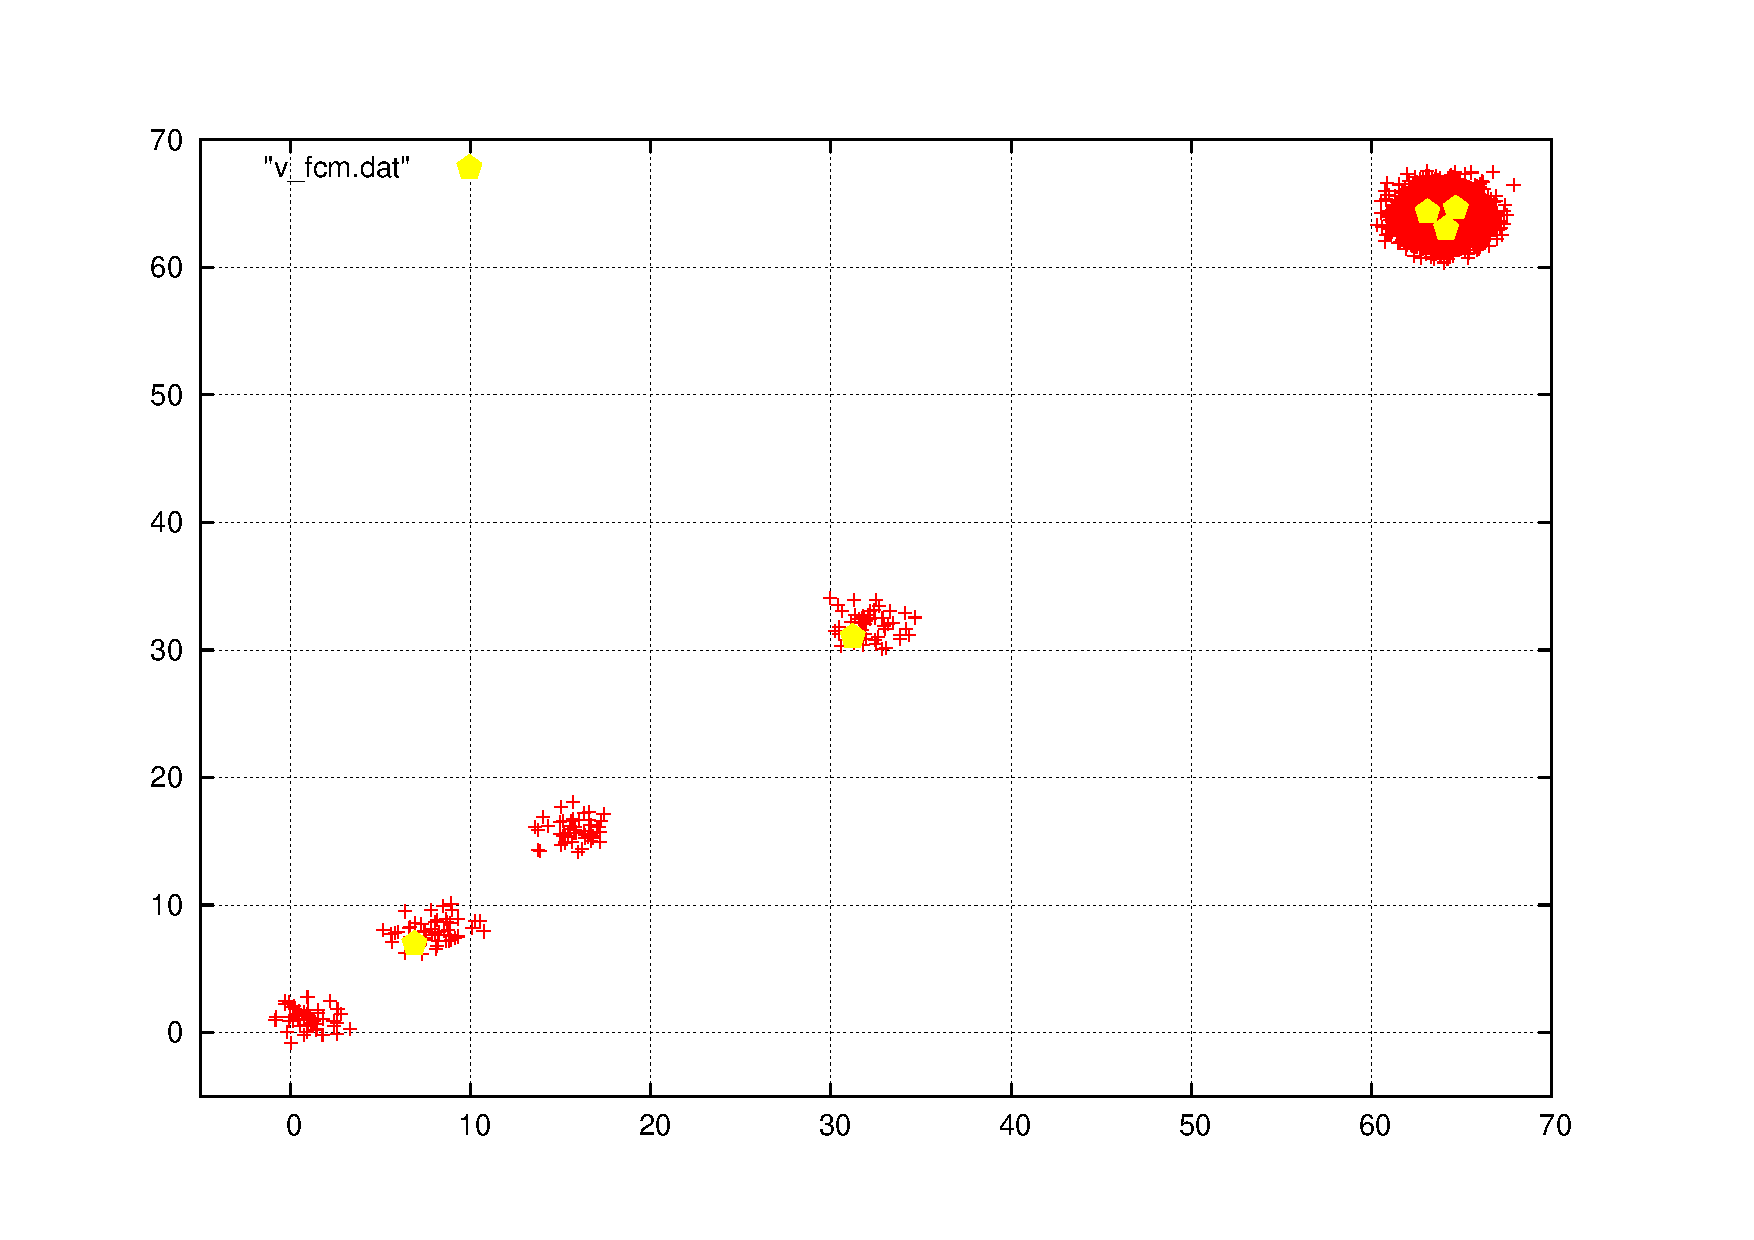
\includegraphics[scale=0.30]{gauss1FCM.pdf}
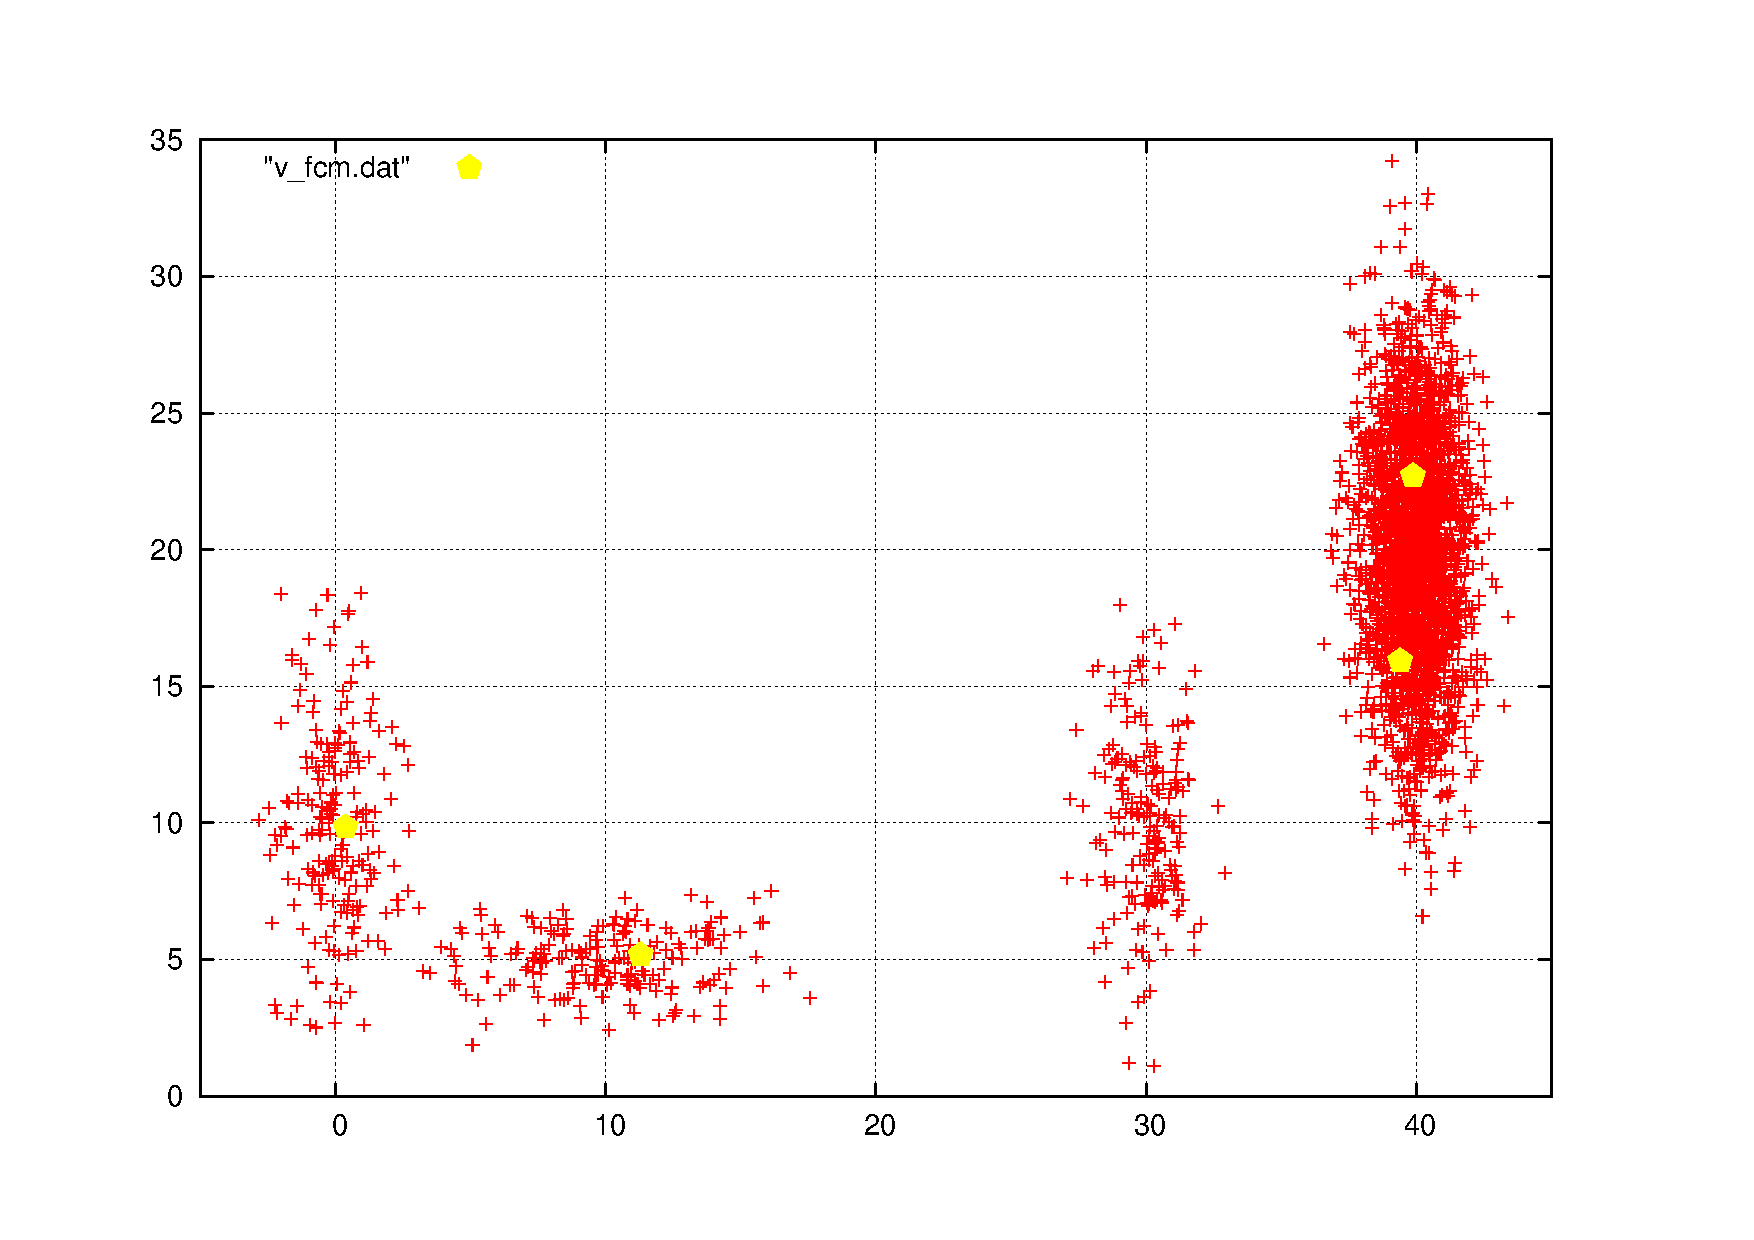
\includegraphics[scale=0.30]{gauss4FCM.pdf}
\end{center}

\section{Optimizing with Differential Evolution}
Differential Evolution is an evolutionary optimization strategy. It uses the principles of evolutionary computation in order to optimize a real-valued objective function.

In DEFC population is made of individuals, each one with its particular disposition of cluster centroids, randomly initialized in space then left to evolve.\\
Differential evolution generates a population of mutating individuals from the existing population of solutions by the process of \emph{mutation} at each of its iterations (named generation)
$$V_{mutant}(c) \longleftarrow V_{p3}(c) + f*(V_{p1}(c)-V_{p2}(c))$$
Vectors which make up the V centroid matrix of a \emph{mutant} individual are constructed starting from three different individuals of the population \emph{p1,p2,p3}. The strength of the mutation is specified by the parameter \emph{f}, which is part of the genome of the individuals and is selected along with the best fit individuals (cfr. jDE)

After the mutation step, chances are the mutant inherits some of the characteristics of the target individual, in the so-called \emph{crossover} process. The emph{crossover ratio} (CR) parameter sets how likely it is for the crossover between the target and the mutant individual to happen. Like the f parameter, also CR parameter is randomly regenerated at each birth of a mutant and brought to the new generation if it contributed successfully in creating a better fit individual.

Final phase of a generation is the \emph{selection} stage. In the selection stage the target individual and the trial individual (name of which was mutant until the crossover step) compete for survival. Fitness values of both are calculated against the objective function, whichever individual sports the lowest value of fitness will take the other's place in the population.\\
The algorithm terminates after a preset number of generations, the best individual's values are returned as result.

\section{Adapting to variable density clusters}
DEFC presented the same problems, although less prominently, as FCM when clustering unbalanced and/or non-globular data (DEFC centroids are shown in black, FCM centroids in yellow).\\

\vspace{-20pt}
\begin{center}
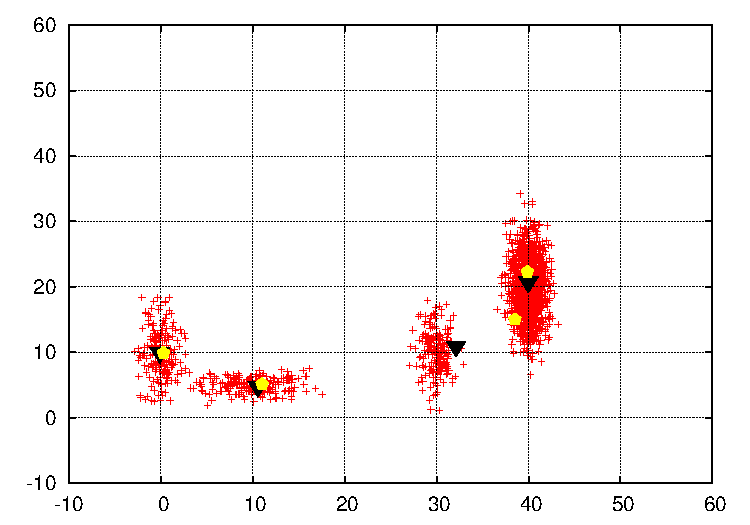
\includegraphics[scale=0.60]{gauss4_mid_full.pdf}
\end{center}

At this point, it was evident that the objective function did not fit this problem very well, so I made a modification to it which adds a reduced scale to the points of very large, very compact clusters.

When the fitness value of an individual is being calculated, a counter is increased each time a point of the input is found to be belonging to the current centroid more than the \emph{counting threshold} value. This is to represent the fact that we consider the point to be more similar to the current centroid than to the others. When the computation of a centroid ends, the counter value is compared to the \emph{cardinality threshold} value which had been generated earlier (more on this in the next paragraph) and if it is greater than the latter the \emph{sigma weight} is applied to the sigma value of the current cluster. This procedure will scale down the contribution of a particularly large cluster, while 

In the initialization phase every individual of the original population is provided with its own randomly generated counting threshold, cardinality threshold and sigma weight values. Then its fitness value is computed.\\
The same happens when a new mutant is generated, so there are many different randomly generated values which will influence for better of for worse the fitness values of the population during evolution. Eventually, the best values will survive along with the host individual as the best fit to solve the problem.\\
Ranges of initialization are [0.5,1] for the counting threshold, [0,n/c] for the cardinality threshold and [0.1,0.9] for the sigma weight.

\section{Experimental results}

\begin{center}
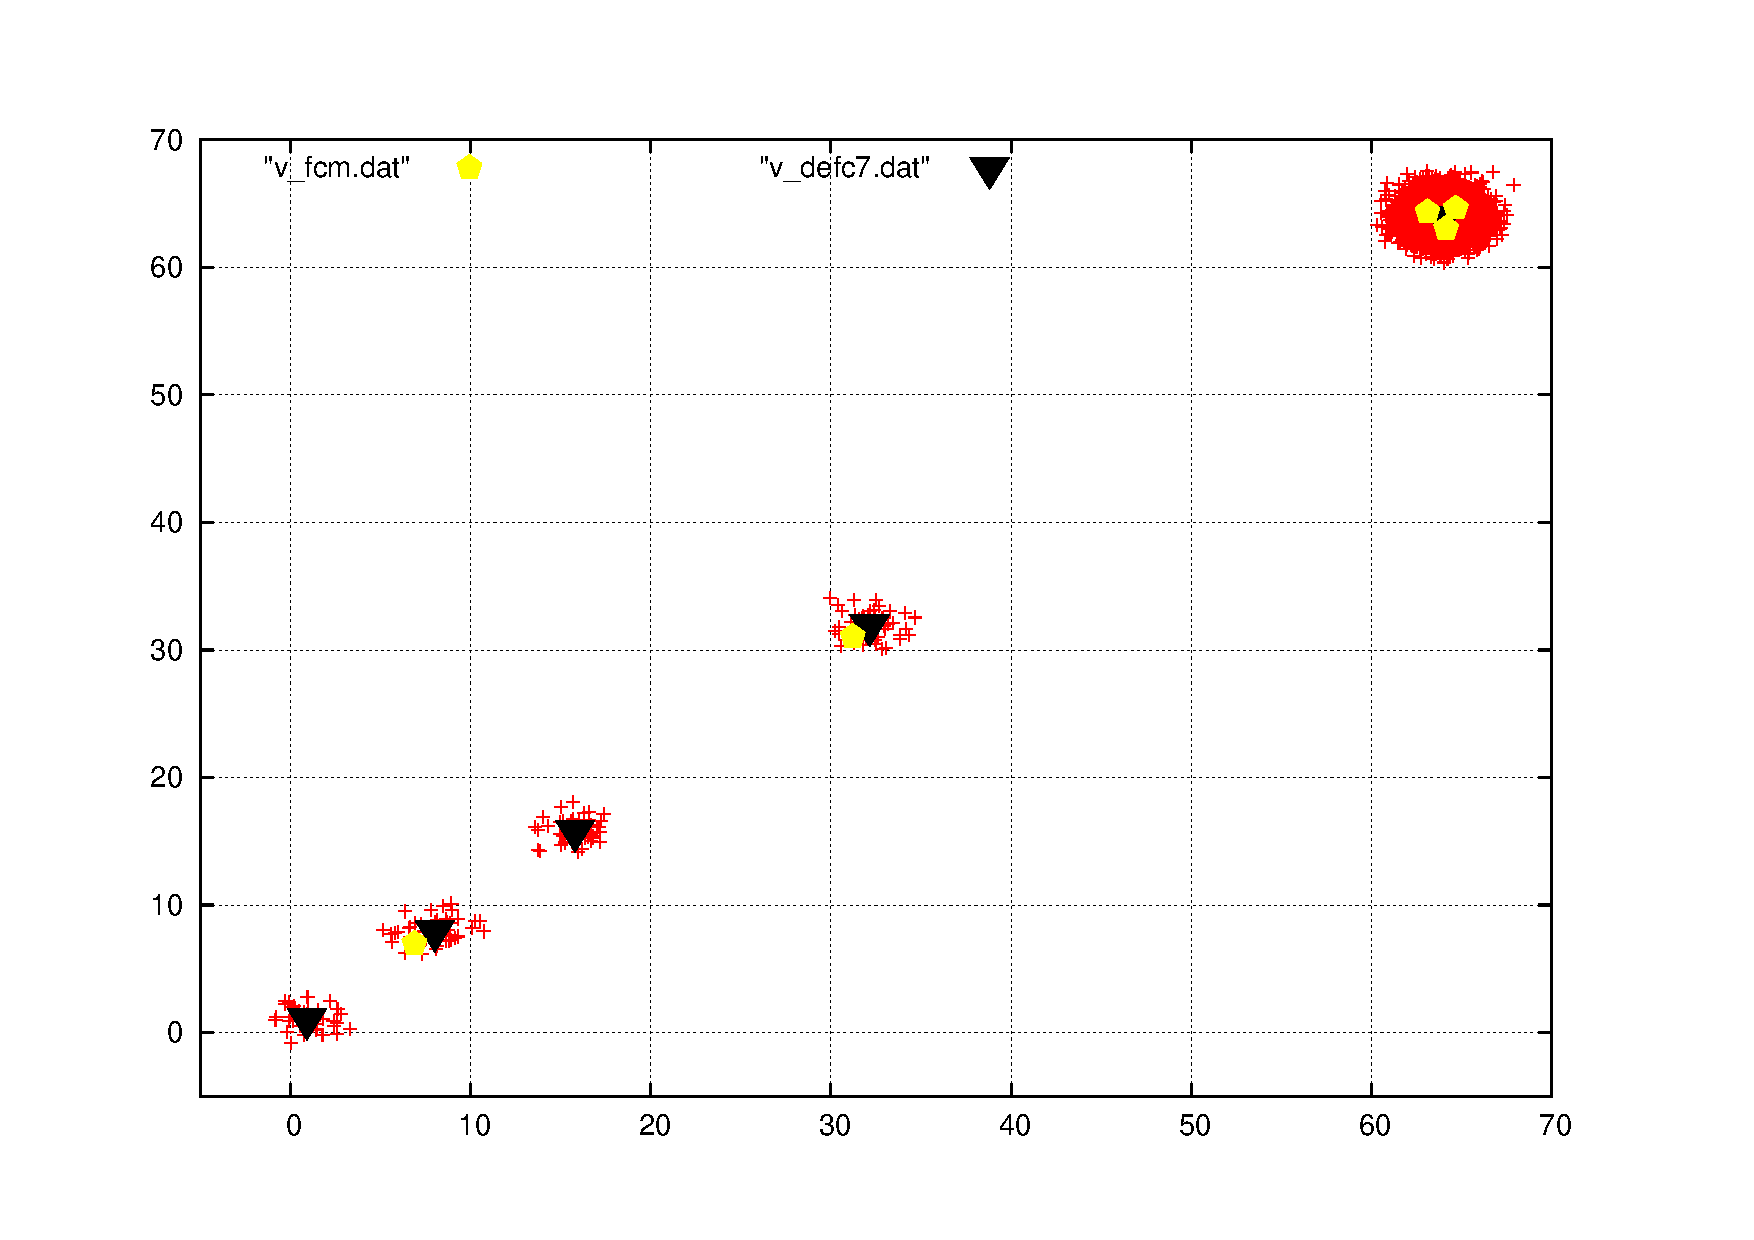
\includegraphics[scale=0.4]{gauss1FINALE.pdf}
\end{center}
\begin{center}
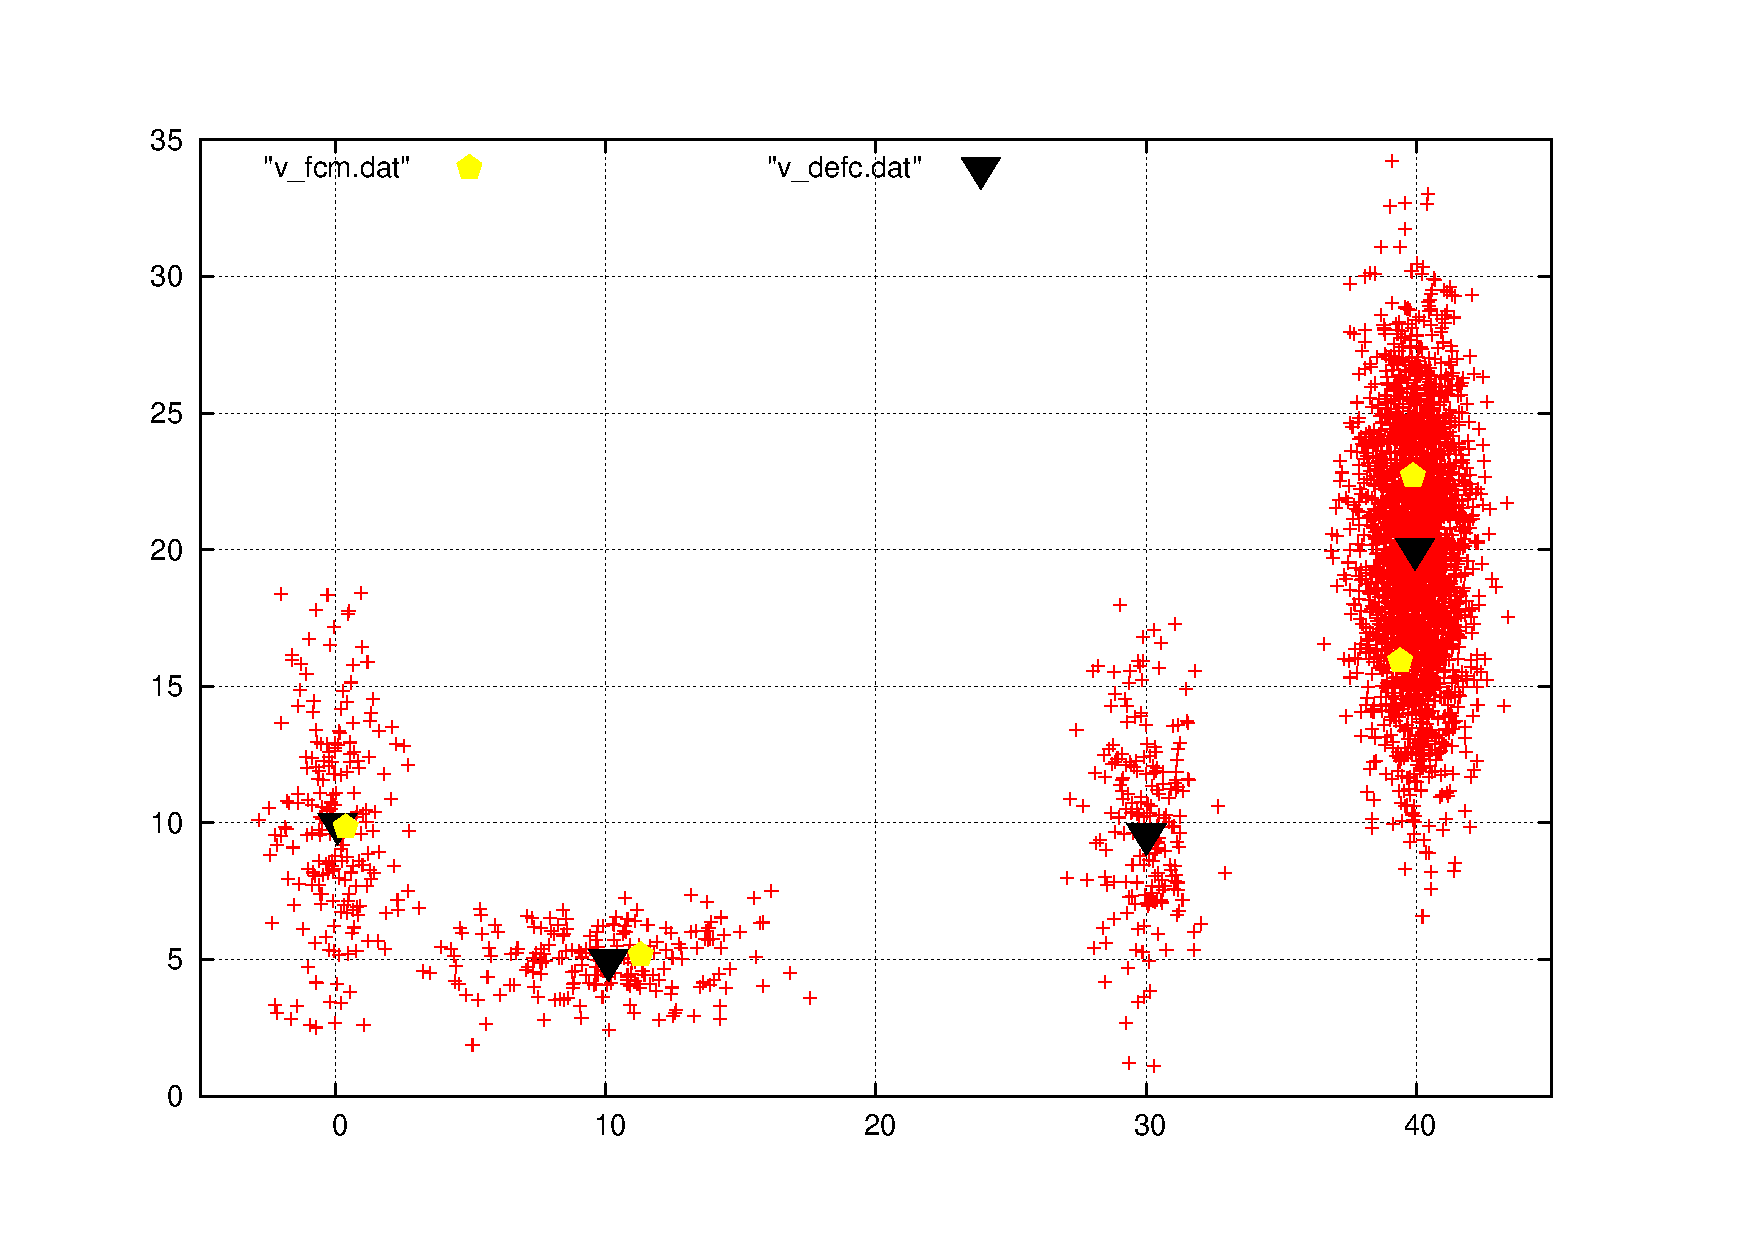
\includegraphics[scale=0.4]{gauss4_finale.pdf}
\end{center}
\begin{center}
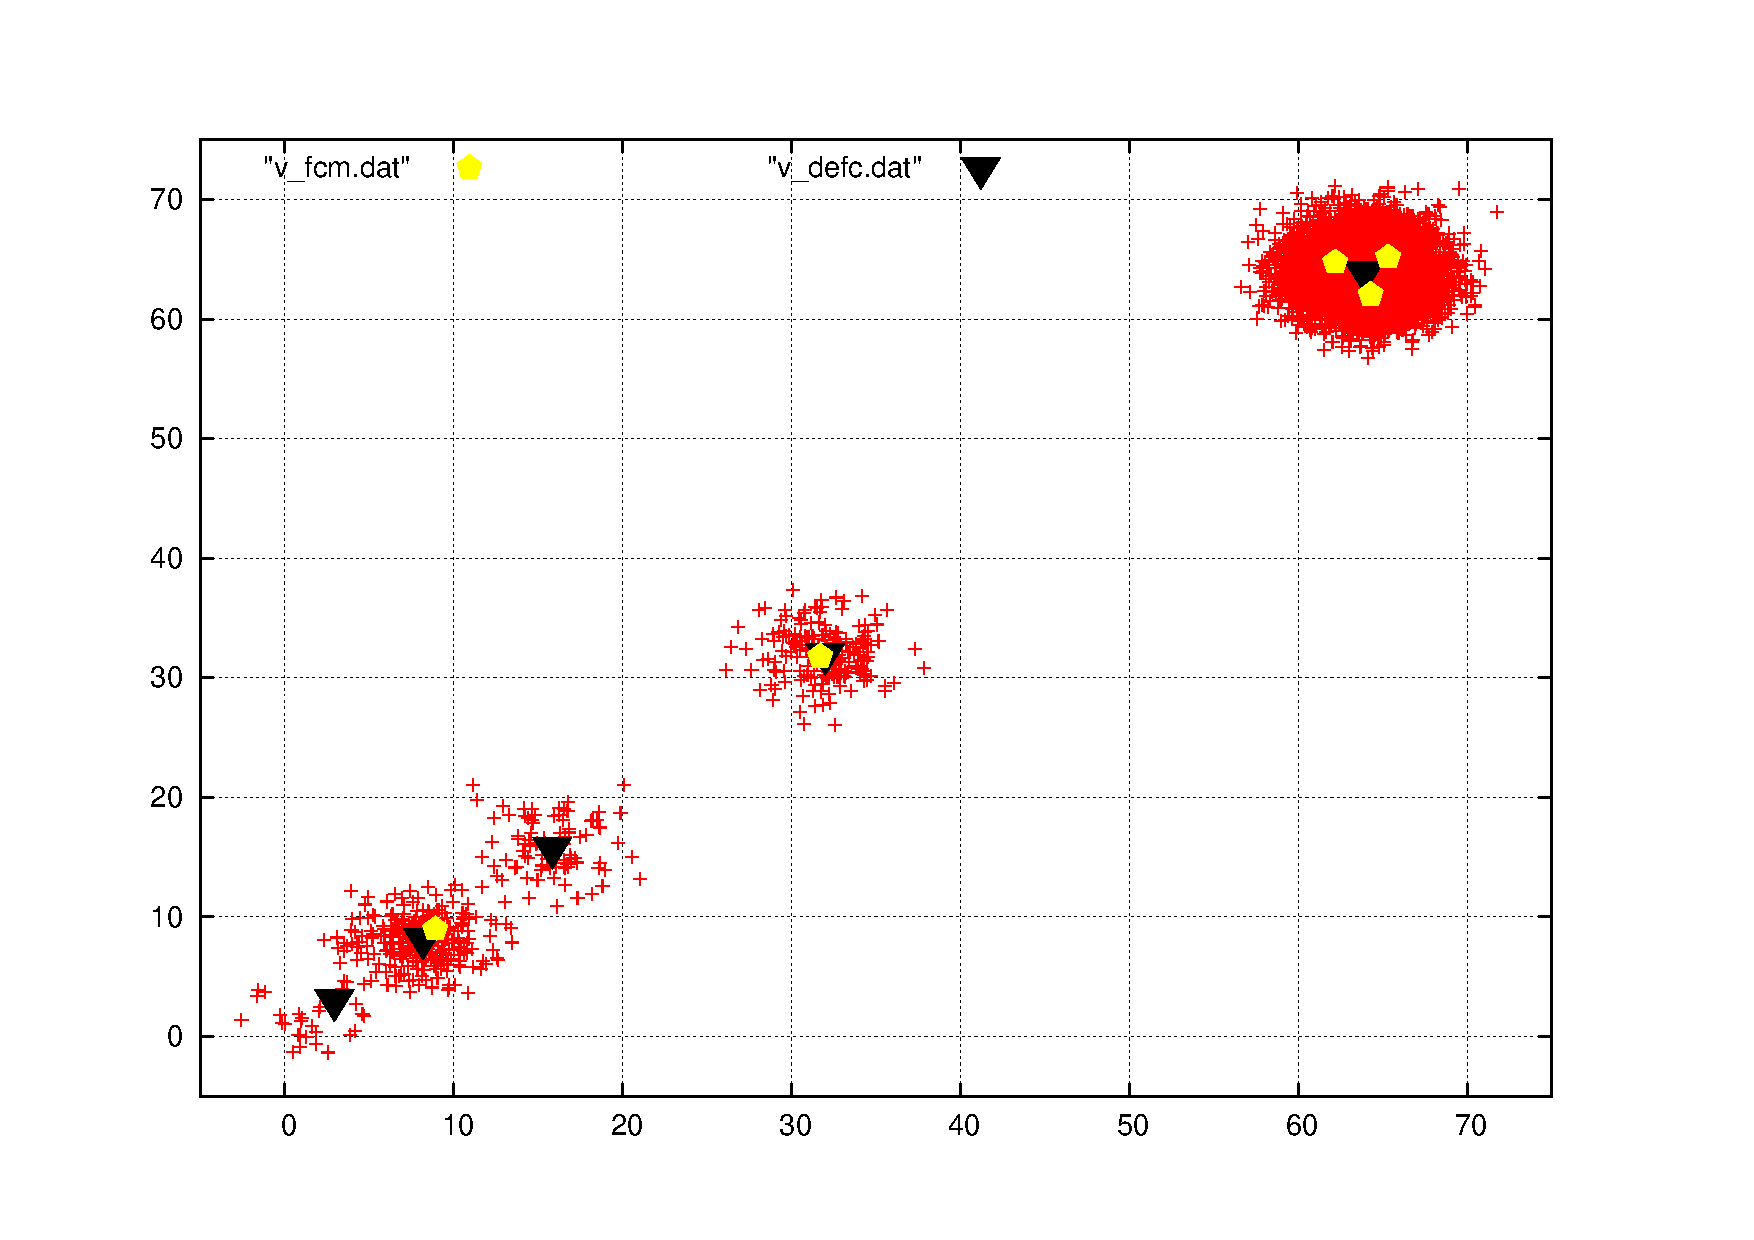
\includegraphics[scale=0.4]{gauss5FINALE.pdf}
\end{center}
\end{document}